    \chapter{Arquitetura e Desenho do Sistema}

A arquitetura de alto nível apresentada na Figura~\ref{fig:top-level} posiciona o \textbf{OmniAI SDK} como o principal resultado deste projeto. Em vez de constituir uma aplicação final isolada, o \textbf{OmniAI SDK} fornece um conjunto de abstrações, componentes e mecanismos reutilizáveis que permitem construir soluções de integração com múltiplos fornecedores de modelos de linguagem de forma consistente. Entre estes componentes encontram-se o domínio comum de pedidos e respostas, os contratos normalizados, os adaptadores responsáveis pela tradução entre o modelo interno e as APIs externas, o \textit{pipeline} de interceptação para funcionalidades transversais e uma DSL de configuração que simplifica a composição do sistema.

A utilização do \textbf{OmniAI SDK} traduz-se, na prática, na criação de uma \textbf{OmniAI Gateway} adaptada às necessidades de cada cenário. A \textbf{Gateway} funciona como um intermediário de acesso unificada sobre diferentes fornecedores de modelos, abstraindo as diferenças existentes entre APIs e disponibilizando uma interface homogénea para clientes e aplicações consumidoras. Desta forma, aspetos relacionados com autenticação, observabilidade, resiliência, encaminhamento de pedidos ou integração com ferramentas externas podem ser configurados ao nível da \textbf{Gateway} sem impactar a lógica das aplicações que a utilizam.

Para validar a arquitetura proposta e demonstrar a aplicabilidade do nosso \textit{Software Development Kit} num cenário real, foi desenvolvida uma instância concreta da \textbf{OmniAI Gateway} como Prova de Conceito (\textit{Proof of Concept} -- PoC). Esta instância é construída integralmente através dos mecanismos disponibilizados pelo \textbf{OmniAI SDK}, recorrendo a configurações declarativas para definir fornecedores, modelos, políticas de autenticação, métricas e restantes componentes da infraestrutura. Durante o arranque da aplicação, estas configurações são utilizadas para compor dinamicamente os adaptadores, a \textit{pipeline} de processamento e os conectores \textbf{HTTP} baseados em \textbf{Ktor} \cite{ktor_ref}, expondo posteriormente um conjunto de \textit{endpoints} compatíveis com os contratos normalizados definidos pelo domínio comum.

Esta separação entre \textbf{OmniAI SDK} e \textbf{OmniAI Gateway} constitui uma das principais decisões arquiteturais do projeto. A biblioteca concentra toda a lógica reutilizável e independente do contexto de execução, enquanto cada \textbf{Gateway} representa uma instanciação específica dessa infraestrutura, podendo ser configurada para diferentes fornecedores, requisitos operacionais ou cenários de utilização sem necessidade de alterar os componentes centrais do sistema.

\begin{figure}[H]
    \centering
    \resizebox{\textwidth}{!}{%
    \begin{tikzpicture}[
        node distance=1.2cm and 1.2cm,
        box/.style={rectangle, draw, rounded corners, align=center, text width=3.8cm, minimum height=1.2cm, inner sep=5pt, thick},
        clientsBox/.style={box, text width=2.5cm},
        entryBox/.style={box, text width=2.0cm},
        sdkBox/.style={box, minimum width=6.0cm, text width=5.5cm, fill=blue!10, minimum height=1.2cm},
        interceptorBox/.style={box, minimum width=2.4cm, text width=2.4cm, minimum height=0.8cm, fill=white},
        group/.style={rectangle, draw, rounded corners, inner sep=15pt, thick},
        arrow/.style={-Latex, thick}
    ]
        % --- CLIENTS ---
        \node[clientsBox] (clients) {Clientes Externos\\ \footnotesize{(Aplicações, REST)}};

        % --- GATEWAY INTERNAL COMPONENTS ---
        \node[entryBox, right=1.2cm of clients] (entry) {Endpoints\\HTTP};
        \node[sdkBox, right=0.6cm of entry] (sdk) {\textbf{OmniAI SDK}\\ \footnotesize{(Core, DSL, Pipeline, Adapters)}};

        \draw[arrow] (entry.east) -- (sdk.west);

        % Interceptors on top of SDK
        \node[interceptorBox, above=0.8cm of sdk, xshift=-1.4cm] (int1) {Interceptor 1};
        \node[interceptorBox, above=0.8cm of sdk, xshift=1.4cm] (int2) {Interceptor 2};

        \draw[arrow] (int1.south) -- (int1.south |- sdk.north);
        \draw[arrow] (int2.south) -- (int2.south |- sdk.north);

        % Grouping them in "Aplicação Gateway"
        \node[group, fit=(entry)(sdk)(int1)(int2), label={[align=center, font=\bfseries]above:Aplicação: OmniAI Gateway}] (gatewayGroup) {};

        \draw[arrow] (clients.east) -- (gatewayGroup.west);

        % --- RIGHT SIDE (External Services) ---
        \node[box, right=1.2cm of gatewayGroup] (providers) {Fornecedores de Inferência\\ \footnotesize{(OpenAI, Anthropic, Gemini)}};
        \node[box, above=0.6cm of providers] (auth) {\textit{Servidor de Autorização}\\ \footnotesize{(OIDC / OAuth2)}};
        \node[box, below=0.6cm of providers] (telemetry) {Observabilidade e Telemetria\\ \footnotesize{(OpenTelemetry)}};

        % Outputs
        \coordinate (fork) at ([xshift=0.5cm]gatewayGroup.east);
        \draw[thick] (gatewayGroup.east) -- (fork);
        \draw[arrow] (fork) |- (auth.west);
        \draw[arrow] (fork) -- (providers.west);
        \draw[arrow] (fork) |- (telemetry.west);

    \end{tikzpicture}%
    }
    \caption{Arquitetura de Alto Nível: O \textbf{OmniAI SDK} utilizado para instanciar uma \textbf{OmniAI Gateway}, abstraindo integrações externas padronizadas.}
    \label{fig:top-level}
\end{figure}

    \begin{figure}[H]
        \centering
        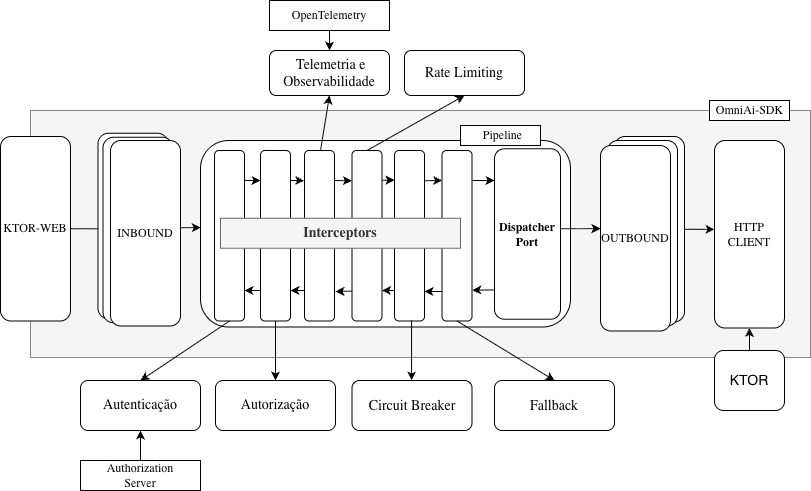
\includegraphics[width=0.95\textwidth]{../images/Arqui}
        \caption{Visão da integração entre \textbf{Ktor}, \textit{inbounds}, \textit{pipeline}, \textit{interceptors}, \textit{outbounds} e \textbf{HTTP} client no \textbf{OmniAI SDK}}
        \label{fig:arquitet-sdk}
    \end{figure}

    A Figura~\ref{fig:top-level} mostra que a \textbf{OmniAI Gateway} não contém a lógica essencial de tradução, despacho ou resiliência. Essa lógica pertence ao \textbf{OmniAI SDK} e é apenas instanciada pela aplicação final. A Figura~\ref{fig:arquitet-sdk} aproxima a visão interna isto é um conector \textbf{HTTP} recebe o corpo do pedido, converte-o para um DTO de contrato, invoca um \textit{inbound adapter}, e este chama um \texttt{DispatcherPort}. A partir desse ponto, a execução pode seguir por um \textit{dispatcher} direto ou por um \textit{dispatcher} apoiado numa \textit{pipeline}. No final, um \textit{outbound adapter} traduz o pedido comum para o contrato do fornecedor e utiliza um cliente \textbf{HTTP} abstrato para executar a chamada real.

    Esta organização permite que aplicações já compatíveis com APIs existentes possam ser integradas com esforço reduzido. Por exemplo, uma aplicação preparada para a API \textbf{Anthropic} pode alterar o seu \texttt{baseURL} para apontar para a \textbf{OmniAI Gateway}, mantendo o contrato esperado pelo cliente. O mesmo princípio aplica-se a clientes compatíveis com a API de inferência da \textbf{OpenAI} e API de inferência do \textbf{Gemini}. 
    
    A arquitetura foi também pensada para escalamento horizontal: o \textbf{OmniAI SDK} evita estado global obrigatório, concentra estado transitório no contexto do pedido e define portas para substituir \textit{stores} em memória por \textit{backends} partilhados quando a \textbf{Gateway} é executada em múltiplas instâncias.

    \section{Modelação do Domínio Comum}

    \subsection{Visão Global do Domínio}

    No final do estudo prévio realizado no capítulo anterior, verificou-se uma acentuada fragmentação estrutural entre os principais fornecedores de Modelos de Linguagem de Grande Escala (LLMs) \cite{ibm_llm_topics}. A ausência de uma padronização ou um protocolo comum leva à inconsistência entre as APIs da \textbf{OpenAI} \cite{openai_api}, \textbf{Anthropic} \cite{anthropic_api} e \textbf{Gemini} \cite{google_gemini_api}, as quais têm campos distintos, diferentes ciclos de vida para o fluxo de dados e estruturas de objetos incompatíveis entre as várias APIs.

    Para garantir a interoperabilidade, a arquitetura do \textbf{OmniAI SDK} assenta na criação de um modelo de domínio comum. A ideia foi criar um modelo de dados interoperável com os maiores fornecedores de inferência para representar pedidos, respostas e eventos dos mesmos, mas sem copiar diretamente a estrutura de nenhum deles.

   Assim, o domínio funciona como um ponto intermédio estável que centraliza qualquer interação no \textbf{OmniAI SDK}. Isto significa que, independentemente de o cliente estruturar o seu pedido original no formato de um fornecedor específico (como por exemplo a \textbf{Anthropic}), esse contrato é imediatamente convertido para o domínio unificado e em seguida, para efetuar a chamada à API, o modelo comum é novamente traduzido para o formato nativo do fornecedor de destino. O mesmo processo inverso ocorre na receção da resposta, os dados que são devolvidos pela API externa são normalizados no nosso domínio comum antes de serem entregues ao cliente na estrutura esperada. Este fluxo completo de transformações está representado visualmente na Figura 3.1.

   
\begin{figure}[H]
    \centering
    \begin{tikzpicture}[
        node distance=0.8cm and 0.5cm,
        % font=\small e larguras ajustadas garantem que o texto não transborda
        box/.style={rectangle, draw, rounded corners, align=center, text width=3.5cm, minimum height=1.2cm, inner sep=4pt, thick, font=\small},
        common/.style={rectangle, draw, rounded corners, align=center, text width=3.2cm, minimum height=1.2cm, inner sep=4pt, fill=gray!20, thick, font=\small},
        api/.style={rectangle, draw, rounded corners, align=center, text width=2.4cm, minimum height=1.2cm, inner sep=4pt, fill=blue!5, dashed, thick, font=\small},
        arrow/.style={-Latex, thick}
    ]
        % --- LINHA DE PEDIDO (Cima) ---
        \node[box] (inReq) {Pedido recebido\\(\textbf{OpenAI}, \textbf{Anthropic}\\ou \textbf{Gemini})};
        \node[common, right=of inReq] (commonReq) {\textbf{CommonRequest}};
        \node[box, right=of commonReq] (contractReq) {Contrato da API\\(\textbf{OpenAI}, \textbf{Anthropic}\\ou \textbf{Gemini})};
        \node[api, right=of contractReq] (apiCall) {Chamada à API\\de Inferência};

        % --- LINHA DE RESPOSTA (Baixo) ---
        \node[api, below=1.2cm of apiCall] (apiResp) {Resposta da API\\de Inferência};
        \node[box, left=of apiResp] (contractResp) {Contrato da API\\(\textbf{OpenAI}, \textbf{Anthropic}\\ou \textbf{Gemini})};
        \node[common, left=of contractResp] (commonResp) {\textbf{CommonResponse}\\ou \textbf{...Event}};
        \node[box, left=of commonResp] (clientResp) {Resposta Cliente\\(\textbf{OpenAI}, \textbf{Anthropic}\\ou \textbf{Gemini})};

        % --- LIGAÇÕES ---
        % Fluxo de Ida
        \draw[arrow] (inReq) -- (commonReq);
        \draw[arrow] (commonReq) -- (contractReq);
        \draw[arrow] (contractReq) -- (apiCall);
        
        % Transição Lógica (Processamento pela API)
        \draw[arrow, dashed] (apiCall) -- (apiResp);

        % Fluxo de Volta
        \draw[arrow] (apiResp) -- (contractResp);
        \draw[arrow] (contractResp) -- (commonResp);
        \draw[arrow] (commonResp) -- (clientResp);
    \end{tikzpicture}
    \caption{Fluxo de normalização entre contratos externos e domínio comum (\textbf{OmniAi-SDK})}
    \label{fig:domain-overview}
\end{figure}

    \subsection{{Estrutura do Domínio Comum}}
    O domínio comum do \textbf{OmniAI SDK} que consite no conjunto de classes e relações que padroniza as interações com os diferentes fornecedores divide-se em dois blocos principais: \textbf{Request} e \textbf{Response}.

    \begin{itemize}
        \item O \textbf{Request} define a estrutura dos pedidos enviados ao modelo.
        \item O \textbf{Response} descreve as respostas devolvidas, quer no formato (\texttt{CommonResponse}), quer em formato incremental através de eventos (\texttt{CommonResponseEvent}).
    \end{itemize}

    \subsubsection{{Modelo Comum de Pedido}}

    O \texttt{CommonRequest} é o modelo base que normaliza qualquer pedido a LLMs, garantindo um contrato único e consistente, independentemente do fornecedor. A estrutura foi desenhada para manter os elementos essenciais de geração (fornecedor, modelo e mensagens) e, ao mesmo tempo, permitir extensões controladas via configuração e opções específicas do \textit{provider}.
    Como se observa na Figura 3.2, o \texttt{CommonRequest} agrega diretamente o \texttt{provider}, o \texttt{model} e a lista de \texttt{messages}, que representam o histórico conversacional. Cada \texttt{CommonRequestMessage} contém o papel (\texttt{CommonRole}) e o conteúdo em partes (\texttt{RequestContentPart}), permitindo combinar texto, JSON ou chamadas a ferramentas. A configuração de geração é isolada em \texttt{CommonGenerationConfig}, enquanto as ferramentas disponíveis são descritas por \texttt{CommonTool} e controladas por \texttt{ToolChoice}. Por fim, \texttt{SystemPrompt} e \texttt{providerOptions} suportam personalizações globais e específicas do fornecedor, mantendo o core estável e extensível.


    \begin{figure}[H]
        \centering
        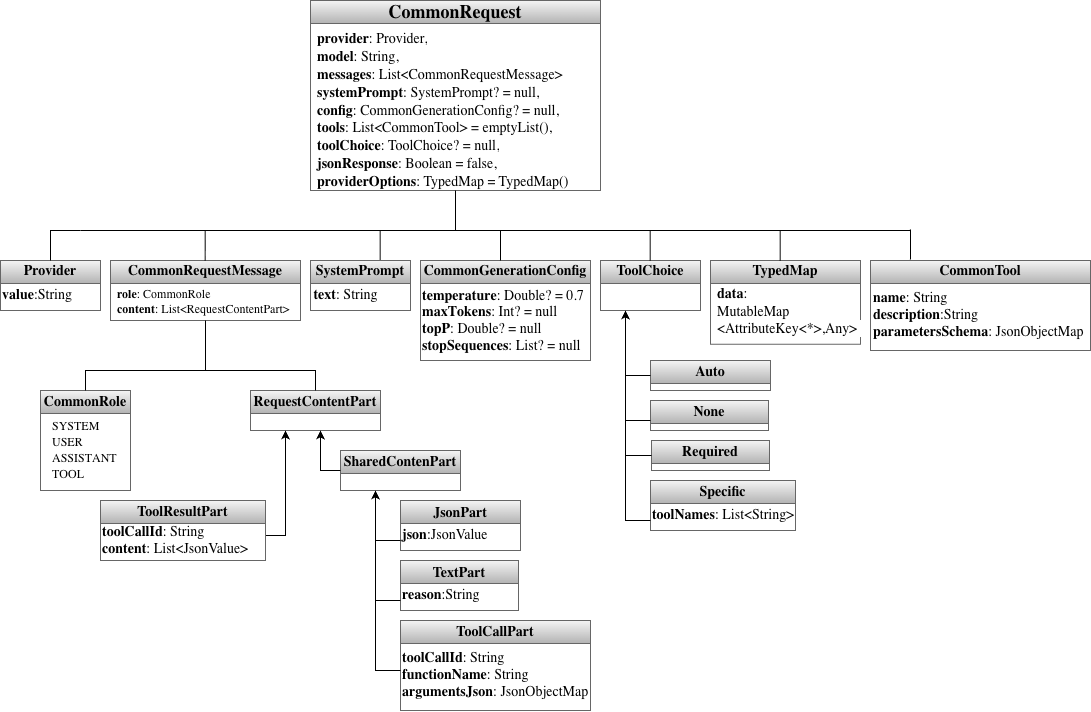
\includegraphics[width=0.95\textwidth]{../images/EstruturaClassesCommonRequestV2}
        \caption{Estrutura de classes do \texttt{CommonRequest}.}
        \label{fig:commonrequest-classes}
    \end{figure}

    Para sistematizar a estrutura apresentada na Figura 3.2, a Tabela~\ref{tab:request-parametros} agrega todos os parâmetros relevantes do domínio de \textit{Request}, incluindo o objeto principal e os tipos diretamente associados. O objetivo é apresentar o significado funcional de cada campo no fluxo de construção do pedido.


    \begin{table}[H]
    \centering
    \scriptsize % Fonte ligeiramente mais pequena para evitar overflow no rodapé
    \setlength{\tabcolsep}{3.5pt} % Menos espaço nas laterais para aproveitar melhor a largura
    \renewcommand{\arraystretch}{1.15}
    \begin{tabularx}{\textwidth}{|>{\raggedright\arraybackslash}p{2.9cm}|>{\raggedright\arraybackslash}p{2.6cm}|>{\raggedright\arraybackslash}p{2.6cm}|>{\raggedright\arraybackslash}X|}
    \hline
    \textbf{Elemento} & \textbf{Campo} & \textbf{Tipo} & \textbf{Descrição} \\ \hline

    CommonRequest & provider & Provider & Fornecedor alvo da chamada. \\ \hline
    CommonRequest & model & String & Identificador do modelo a utilizar. \\ \hline
    CommonRequest & messages & List<Common\-RequestMessage> & Histórico de mensagens enviado ao modelo. \\ \hline
    CommonRequest & systemPrompt & SystemPrompt? & Prompt de sistema global (opcional). \\ \hline
    CommonRequest & config & Common\-GenerationConfig? & Parâmetros de geração (opcional). \\ \hline
    CommonRequest & tools & List<CommonTool> & Ferramentas disponíveis para chamadas de função. \\ \hline
    CommonRequest & toolChoice & ToolChoice? & Política de seleção de ferramentas. \\ \hline
    CommonRequest & jsonResponse & Boolean & Indica se a resposta deve ser forçada a JSON. \\ \hline
    CommonRequest & providerOptions & TypedMap & Opções específicas do fornecedor. \\ \hline

    CommonRequest\-Message & role & CommonRole & Papel da mensagem (SYSTEM, USER, ASSISTANT, TOOL). \\ \hline
    CommonRequest\-Message & content & List<Request\-ContentPart> & Conteúdo segmentado da mensagem. \\ \hline

    SystemPrompt & text & String & Conteúdo do prompt de sistema. \\ \hline

    Common\-GenerationConfig & temperature & Double? & Grau de aleatoriedade da geração. \\ \hline
    Common\-GenerationConfig & maxTokens & Int? & Limite máximo de \textit{tokens} de saída. \\ \hline
    Common\-GenerationConfig & topP & Double? & Probabilidade cumulativa. \\ \hline
    Common\-GenerationConfig & stopSequences & List<String>? & Sequências que interrompem a geração. \\ \hline

    CommonTool & name & String & Nome da ferramenta. \\ \hline
    CommonTool & description & String & Descrição funcional da ferramenta. \\ \hline
    CommonTool & parametersSchema & JsonObjectMap & Esquema JSON dos parâmetros. \\ \hline

    ToolChoice & Auto / None / Required / Specific & -- & Estratégia de uso de ferramentas (auto, nenhuma, obrigatório ou lista específica). \\ \hline
    ToolChoiceAuto & -- & -- & Subtipo sem campos (seleção automática). \\ \hline
    ToolChoiceNone & -- & -- & Subtipo sem campos (sem ferramentas). \\ \hline
    ToolChoiceRequired & -- & -- & Subtipo sem campos (uso obrigatório). \\ \hline
    ToolChoiceSpecific & toolNames & List<String> & Lista de ferramentas permitidas. \\ \hline

    Provider & value & String & Identificador textual do fornecedor. \\ \hline
    TypedMap & data & Map<String, Any?> & Mapa genérico de opções específicas do fornecedor. \\ \hline

    RequestContentPart & TextPart & text: String & Conteúdo textual. \\ \hline
    RequestContentPart & JsonPart & json: JsonValue & Conteúdo JSON estruturado. \\ \hline
    RequestContentPart & ToolCallPart & toolCallId,\newline functionName,\newline argumentsJson & Chamada a ferramenta com argumentos. \\ \hline
    RequestContentPart & ToolResultPart & toolCallId,\newline content & Resultado de execução de ferramenta. \\ \hline

    \end{tabularx}
    \caption{Parâmetros do domínio de \textit{Request}.}
    \label{tab:request-parametros}
\end{table}


    \subsubsection{{Modelo Comum de Resposta e Eventos}}

    O \texttt{CommonResponse} é o modelo base que normaliza as respostas devolvidas pelos diferentes fornecedores, garantindo um contrato único e consistente para o cliente. A estrutura foi desenhada para representar o resultado final da geração, mantendo as escolhas (\texttt{CommonChoice}) com o respetivo índice e a razão de término (\texttt{FinishReason}). Cada escolha contém uma mensagem (\texttt{CommonResponseMessage}) com o papel (\texttt{CommonRole}) e o conteúdo em partes (\texttt{Response\allowbreak Content\allowbreak Part}), permitindo combinar texto, JSON, chamadas a ferramentas ou recusas. A informação de uso (\texttt{CommonUsage}) isola o consumo de \textit{tokens} e facilita métricas e contabilização. Por fim, \texttt{providerOptions} preserva metadados específicos do fornecedor, mantendo o núcleo do domínio estável e extensível.

    \begin{figure}[H]
        \centering
        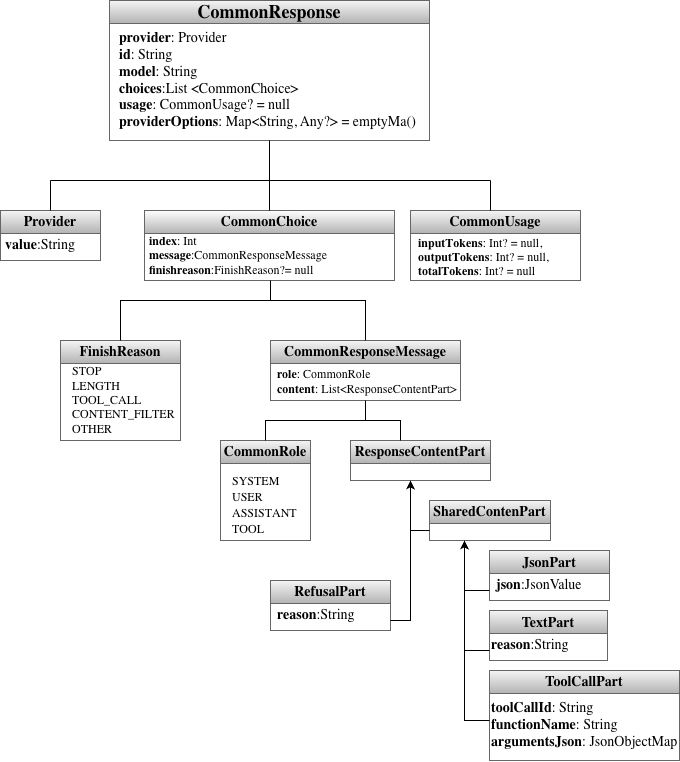
\includegraphics[width=0.95\textwidth]{../images/EstruturaClassesCommonResponseV2.drawio.png}
        \caption{Estrutura de classes do \texttt{CommonResponse}.}
        \label{fig:commonresponse-classes}
    \end{figure}

    A Tabela~\ref{tab:response-parametros} reúne os campos do domínio de \textit{Response}, incluindo o objeto base, as escolhas e os eventos de \textit{streaming}.

        \begin{table}[H]
    \centering
    \scriptsize
    \setlength{\tabcolsep}{4pt}
    \renewcommand{\arraystretch}{1.2}
    \begin{tabularx}{\textwidth}{|>{\raggedright\arraybackslash}p{3.4cm}|>{\raggedright\arraybackslash}p{2.2cm}|>{\raggedright\arraybackslash}p{3.8cm}|>{\raggedright\arraybackslash}X|}
        \hline
        \textbf{Elemento} & \textbf{Campo} & \textbf{Tipo} & \textbf{Descrição} \\ \hline

        CommonResponse & \textit{provider} & Provider & Fornecedor que produziu a resposta. \\ \hline
        CommonResponse & id & String & Identificador do pedido/execução. \\ \hline
        CommonResponse & model & String & Identificador do modelo utilizado. \\ \hline
        CommonResponse & choices & List<CommonChoice> & Lista de escolhas geradas. \\ \hline
        CommonResponse & usage & CommonUsage? & Contabilização de \textit{tokens} (opcional). \\ \hline
        CommonResponse & providerOptions & Map<String, Any?> & Metadados específicos do fornecedor. \\ \hline

        CommonChoice & index & Int & Índice da escolha. \\ \hline
        CommonChoice & message & CommonResponseMessage & Mensagem com papel e conteúdo. \\ \hline
        CommonChoice & finishReason & FinishReason? & Razão de término da escolha (opcional). \\ \hline

        CommonResponseMessage & role & CommonRole & Papel da mensagem. \\ \hline
        CommonResponseMessage & content & List<ResponseContentPart> & Conteúdo segmentado da resposta. \\ \hline

        CommonUsage & inputTokens & Int? & Tokens de entrada. \\ \hline
        CommonUsage & outputTokens & Int? & Tokens de saída. \\ \hline
        CommonUsage & totalTokens & Int? & Total de \textit{tokens}. \\ \hline

        % Correção solicitada: O enum foi para a coluna 'Tipo' e formatado com quebras limpas
        FinishReason & -- & STOP / LENGTH / \newline TOOL\_CALL / \newline CONTENT\_FILTER / \newline OTHER & Motivo de conclusão da geração. \\ \hline

        ResponseContentPart & TextPart & text: String & Segmento textual. \\ \hline
        ResponseContentPart & JsonPart & json: JsonValue & Segmento JSON estruturado. \\ \hline
        ResponseContentPart & ToolCallPart & toolCallId, \newline functionName, \newline argumentsJson & Chamada a ferramenta. \\ \hline
        ResponseContentPart & RefusalPart & reason: String & Recusa do modelo com justificação. \\ \hline

    \end{tabularx}
    \caption{Parâmetros do domínio de \textit{Response} (CommonResponse).}
    \label{tab:response-parametros}
\end{table}

    O \texttt{CommonResponseEvent} complementa o \texttt{CommonResponse} ao representar respostas em \textit{streaming} como uma sequência ordenada de eventos. Esta abordagem permite construir a saída de forma incremental: primeiro sinaliza o início da resposta, depois o arranque de cada escolha, segue com deltas de texto ou de argumentos de ferramentas e, por fim, reporta o fecho da escolha, o uso de \textit{tokens} e a conclusão (ou erro) do \textit{stream}. Cada evento partilha um conjunto mínimo de metadados (fornecedor, identificador, modelo e sequência) que asseguram consistência e reordenação determinística.

    \begin{table}[H]
    \centering
    \scriptsize
    \setlength{\tabcolsep}{4pt}
    \renewcommand{\arraystretch}{1.2}
    \begin{tabularx}{\textwidth}{|>{\raggedright\arraybackslash}p{3.5cm}|>{\raggedright\arraybackslash}p{2.5cm}|>{\raggedright\arraybackslash}p{2.0cm}|>{\raggedright\arraybackslash}X|}
        \hline
        \textbf{Elemento} & \textbf{Campo} & \textbf{Tipo} & \textbf{Descrição} \\ \hline

        CommonResponse\newline Event & \textit{provider} & Provider & Fornecedor associado ao evento. \\ \hline
        CommonResponse\newline Event & id & String & Identificador do pedido/execução. \\ \hline
        CommonResponse\newline Event & model & Model & Modelo utilizado no evento. \\ \hline
        CommonResponse\newline Event & sequence & Long & Ordem do evento no \textit{stream}. \\ \hline
        CommonResponse\newline Event & \textit{provider}\newline EventType & String? & Tipo bruto do evento do fornecedor (opcional). \\ \hline

        ResponseStarted & -- & -- & Início do \textit{streaming} da resposta. \\ \hline

        ChoiceStarted & choiceIndex & Int & Índice da escolha iniciada. \\ \hline
        ChoiceStarted & role & CommonRole? & Papel associado à escolha (opcional). \\ \hline

        TextDeltaEvent & choiceIndex & Int & Índice da escolha que recebe o delta. \\ \hline
        TextDeltaEvent & text & String & Fragmento incremental de texto. \\ \hline

        ToolCall\newline StartedEvent & choiceIndex & Int & Índice da escolha. \\ \hline
        ToolCall\newline StartedEvent & toolCallIndex & Int & Índice da chamada a ferramenta. \\ \hline
        ToolCall\newline StartedEvent & toolCallId & String & Identificador da chamada a ferramenta. \\ \hline
        ToolCall\newline StartedEvent & functionName & String & Nome da função invocada. \\ \hline

        ToolCallArguments\newline DeltaEvent & choiceIndex & Int & Índice da escolha. \\ \hline
        ToolCallArguments\newline DeltaEvent & toolCallIndex & Int & Índice da chamada a ferramenta. \\ \hline
        ToolCallArguments\newline DeltaEvent & arguments\newline Fragment & String & Fragmento incremental de argumentos. \\ \hline

        ChoiceFinished & choiceIndex & Int & Índice da escolha terminada. \\ \hline
        ChoiceFinished & finishReason & FinishReason? & Razão de término (opcional). \\ \hline

        UsageReported & usage & CommonUsage & Contabilização de \textit{tokens} reportada. \\ \hline

        ResponseCompleted & -- & -- & Conclusão do \textit{streaming} da resposta. \\ \hline

        ResponseErrored & message & String & Mensagem de erro. \\ \hline
        ResponseErrored & retryable & Boolean & Indica se o erro é recuperável. \\ \hline

    \end{tabularx}
    \caption{Parâmetros do domínio de \textit{Response} (CommonResponseEvent).}
    \label{tab:response-events-parametros}
\end{table}

    \subsection{{Mapa Tipificado e Extensibilidade do Domínio}}
    Nem todos os dados relevantes pertencem ao modelo mínimo de inferência. Algumas informações são específicas do fornecedor, como parâmetros avançados do \textbf{Gemini} e outras pertencem ao contexto operacional, como metadados de autenticação, IP do cliente, cabeçalhos \textbf{HTTP} ou atributos necessários para observabilidade e autorização. Para estes casos, o \textbf{OmniAI SDK} introduz a estrutura \texttt{TypedMap}.

O \texttt{TypedMap} funciona como um mapa de atributos tipado por chave. Cada \texttt{AttributeKey<T>} associa um nome lógico a um tipo esperado, permitindo guardar e recuperar valores sem depender de conversões frágeis de strings. Esta abordagem é mais segura do que um \texttt{Map<String, Any?>} puro, porque cada chave transporta também a expectativa de tipo. Ao mesmo tempo, é mais flexível do que adicionar campos ao domínio sempre que surge uma necessidade nova.

\begin{figure}[H]
    \centering
    \resizebox{0.9\textwidth}{!}{%
        \begin{tikzpicture}[
            node distance=1.1cm and 1.0cm,
            box/.style={rectangle, draw, rounded corners, align=center, minimum width=3.4cm, minimum height=0.9cm},
            map/.style={rectangle, draw, rounded corners, align=left, minimum width=5.0cm, minimum height=2.7cm, fill=gray!10},
            arrow/.style={-Latex, thick}
        ]
            \node[box] (auth) {Metadados de autenticação};
            \node[box, below=of auth] (http) {Cabeçalhos e IP do cliente};
            \node[box, below=of http] (provider) {Opções específicas do fornecedor};

            \node[map, right=2.0cm of http] (typedmap) {\texttt{TypedMap}\\[0.2cm]
            \texttt{AttributeKey<String>}\\
            \texttt{AttributeKey<AuthResult>}\\
            \texttt{AttributeKey<Set<String>>}\\
            \texttt{AttributeKey<Int>}};

            \node[box, right=2.0cm of typedmap] (consumers) {Componentes do \textbf{SDK}\\ leem atributos tipados};

            \draw[arrow] (auth.east) -- (typedmap.west);
            \draw[arrow] (http.east) -- (typedmap.west);
            \draw[arrow] (provider.east) -- (typedmap.west);
            \draw[arrow] (typedmap.east) -- (consumers.west);
        \end{tikzpicture}}
    \caption{Utilização da \texttt{TypedMap} para transportar atributos extensíveis}
    \label{fig:typed-map}
\end{figure}

No domínio de inferência, a \texttt{TypedMap} aparece em \texttt{providerOptions}, permitindo preservar dados que não pertencem ao subconjunto comum mas não devem ser perdidos durante a tradução. Fora da inferência estrita, a mesma estrutura permite transportar metadados entre componentes sem criar dependências diretas entre eles. Esta característica é útil para a evolução futura do \textbf{OmniAI SDK}, porque permite que mecanismos ,como autorização, observabilidade ou políticas de execução, usem atributos adicionais sem forçar alterações constantes nas classes centrais do domínio.
    


\section{Arquitetura do Sistema}

A Arquitetura Hexagonal, também conhecida como padrão de Portas e Adaptadores, foi escolhida neste projeto para garantir que a lógica principal do sistema permaneça independente de detalhes técnicos e de integrações externas. Em vez de o \textit{core} da aplicação depender diretamente de bibliotecas, protocolos ou APIs específicas, toda a comunicação com o exterior acontece através de interfaces bem definidas, enquanto os adaptadores tratam das implementações concretas \cite{gfg_hexagonal_architecture, hexagonal_ports, netflix_hexagonal}.

Esta separação torna-se especialmente importante no contexto de uma \textit{Gateway} de Inteligência Artificial, uma vez que o sistema atua como ponto central de comunicação entre clientes \textbf{HTTP}, fornecedores de inferência, mecanismos de autenticação e serviços de observabilidade. Sem um isolamento arquitetural claro, a lógica de domínio acabaria inevitavelmente dependente de \textit{SDKs} externos, formatos proprietários e detalhes específicos de integração de cada fornecedor.

Ao adotar esta abordagem, foi possível manter o \textit{core} do \textbf{OmniAI SDK} focado apenas nas responsabilidades centrais de normalização, abstração e coordenação. Assim, funcionalidades como chamadas de rede, serialização de dados ou integração com APIs externas ficam confinadas aos adaptadores. Isto permite que novos fornecedores de IA, novos mecanismos de autenticação e outros mecanismos sejam adicionados com alterações mínimas na lógica principal da aplicação.

Durante o desenho da solução, foram analisadas outras abordagens arquiteturais para avaliar qual delas se ajustava melhor aos requisitos do projeto. Uma das alternativas consideradas foi a arquitetura tradicional em camadas. Apesar de ser uma solução mais simples numa fase inicial, este modelo tende a perder clareza estrutural à medida que o sistema cresce. Com o tempo, torna-se comum encontrar regras de negócio misturadas com lógica de transporte, chamadas \textbf{HTTP} e tratamento de contratos externos, aumentando o acoplamento e dificultando a manutenção \cite{graca_explicit_architecture}.

Neste contexto, a Arquitetura Hexagonal revelou-se a solução mais adequada para os objetivos do projeto. A abordagem oferece modularidade, isolamento e flexibilidade suficientes para lidar com as diferentes políticas transversais exigidas por uma \textit{Gateway} de Inteligência Artificial, como autenticação, resiliência, observabilidade e roteamento de pedidos, mantendo ao mesmo tempo uma estrutura organizada e simples de evoluir \cite{api_gateway_design, ai_gateway_pattern, karl_ai_gateway}. Além disso, esta organização arquitetural facilita a introdução de novos fornecedores e novas funcionalidades sem comprometer a estabilidade do núcleo da aplicação.

    \subsection{Contratos}
    Os módulos \texttt{contracts:openai}, \texttt{contracts:anthropic} e \texttt{contracts:gemini} modelam os formatos de pedido, resposta e eventos de cada fornecedor. Estes contratos são DTOs no sentido em que representam dados transportados na fronteira do sistema, mas não são apenas DTOs genéricos. São chamados \textit{contracts} porque codificam uma compatibilidade externa concreta: nomes de campos, estruturas JSON, eventos de \textit{streaming}, campos opcionais, formatos de erro e convenções específicas de cada API.

    Esta distinção é importante. Um DTO interno poderia ser livremente alterado sem impacto externo um contrato compatível com \textbf{OpenAI}, \textbf{Anthropic} ou \textbf{Gemini} precisa de respeitar o formato que clientes e fornecedores esperam. Ao isolar estes contratos em módulos próprios, o \textbf{OmniAI SDK} evita que detalhes como \texttt{tool\_calls}, \texttt{content\_block\_delta} ou \texttt{functionDeclarations} se espalhem pelo domínio comum.

    \subsection{Adaptadores de Entrada}
    Os adaptadores de entrada recebem pedidos no formato do cliente e traduzem-nos para \texttt{CommonRequest}. Cada \textit{inbound} implementa a porta \texttt{InboundPort} e recebe um \texttt{DispatcherPort}, não uma implementação concreta de \textit{pipeline} ou de fornecedor. Além disso, cada \textit{inbound} usa uma implementação de \texttt{InboundTranslator}, responsável por converter o objeto de entrada para domínio e por converter a resposta comum de volta para o contrato do cliente.

    Esta decisão evita que o \textit{inbound} exponha diretamente uma Web API. O \textbf{OmniAI SDK} fornece \textit{adapters} que trabalham sobre DTO's, e a exposição \textbf{HTTP} fica noutro \textit{adapter}, como o \texttt{gateway-ktor-server} (detalhado na Secção~\ref{sec:gateway-ktor-server}). Assim, um servidor \textbf{Ktor}, uma função serverless, um \textit{handler} Express ou outro mecanismo de entrada podem chamar o mesmo \textit{inbound} desde que consigam construir o DTO esperado. Esta separação reduz a dependência do domínio e dos \textit{inbounds} face a bibliotecas \textbf{HTTP} externas.

    \subsection{Adaptadores de Saída}
    Os adaptadores de Saída fazem o caminho inverso: recebem um \texttt{CommonRequest}, traduzem-no para o contrato do fornecedor real e executam a chamada externa. Cada \textit{outbound} implementa \texttt{OutboundPort}, identifica \texttt{provider}, \texttt{model} e \texttt{key}, e delega a tradução num \texttt{OutboundTranslator}. A implementação atual inclui \textit{outbounds} para \textbf{OpenAI}, \textbf{Anthropic} e \textbf{Gemini}.

    Ao contrário dos \textit{inbounds}, os \textit{outbounds} precisam de comunicar com serviços externos. Por isso, recebem uma implementação de \texttt{HttpTransportClient}, a porta de transporte \textbf{HTTP} descrita na Secção~\ref{subsec:http-transport-client}, que abstrai por completo o mecanismo de rede utilizado. Esta inversão de dependência é o que permite testar \textit{adapters} sem depender de chamadas reais e evoluir o ambiente de execução sem reescrever o domínio.

    \subsection{Camada de Comunicação HTTP}
    \label{subsec:http-transport-client}

    A interface \texttt{HttpTransportClient}, definida no módulo \texttt{core}, representa a porta de saída responsável por toda a comunicação \textbf{HTTP} do nosso \textbf{SDK} com os fornecedores externos. Esta abstração isola completamente os \textit{outbound adapters} de qualquer biblioteca ou mecanismo concreto de rede, seguindo o princípio de inversão de dependência que caracteriza a Arquitetura Hexagonal.

    A interface expõe três operações distintas. A operação \texttt{execute} é utilizada para pedidos síncronos: recebe uma configuração tipificada de pedido (\texttt{RequestConfig}) e um serializador, executa a chamada \textbf{HTTP} e devolve um \texttt{HttpCallResult}. A operação \texttt{listen} destina-se a respostas em \textit{streaming} baseadas em \textit{Server-Sent Events} (\textbf{SSE}) com um único tipo de evento, devolvendo um \texttt{Flow} de resultados. A operação \texttt{listenMany} generaliza o modelo de \textbf{SSE} para cenários com múltiplos tipos de eventos, selecionando o serializador adequado com base no campo \texttt{event} de cada mensagem.

    O resultado de qualquer chamada \textbf{HTTP} é representado pela classe selada \texttt{HttpCallResult}, parametrizada pelo tipo da resposta esperada. Esta classe cobre os seguintes casos: \texttt{Success}, que encapsula os dados desserializados; \texttt{ApiError}, que retém o código de estado \textbf{HTTP} e o corpo da resposta de erro; \texttt{NetworkError}, originado por falhas de conectividade; \texttt{SerializationError}, resultante de respostas com formato inesperado; e \texttt{UnknownError}, para situações não classificadas. Todos os casos carregam um \texttt{TypedMap} de metadados, que permite propagar cabeçalhos de resposta e outras informações contextuais para os adaptadores e intercetores de forma estruturada.

    A implementação concreta desta interface é descrita na Secção~\ref{sec:ktor-transport-impl}.

    \subsection{Dispatcher}
    O \texttt{DispatcherPort} é a porta chamada pelos \textit{inbounds} para executar um \texttt{CommonRequest}. A sua responsabilidade não é, por si só, conter inteligência de roteamento; é despachar o pedido para uma estratégia de execução. No \textbf{OmniAI SDK} é fornecida uma implementação simples, criada por \texttt{routingDispatcherFactory}, que procura o \textit{outbound} cujo \texttt{provider} e \texttt{model} correspondem aos campos do pedido e envia a chamada para esse \textit{adapter}.

    Como se trata de uma interface, a arquitetura permite outras implementações com objetivos diferentes. Um consumidor do \textbf{SDK} pode fornecer um \textit{dispatcher} direto, um \textit{dispatcher} com seleção por custo, um \textit{dispatcher} que consulta políticas externas ou um \textit{dispatcher} que aplica regras mais complexas. A \textit{pipeline} fornecida pelo \textbf{SDK} é ela própria encaixada através de um \textit{adapter}, \texttt{PipelineBackedDispatcher}, preservando a ideia de que os \textit{inbounds} dependem apenas de \texttt{DispatcherPort}.

    \section{Organização do \textit{\textbf{SDK}}}
    O \textbf{SDK} está organizado como um projeto \textbf{Gradle} multi-módulo. Os módulos principais incluem \texttt{core}, \texttt{contracts}, \texttt{inbound}, \texttt{outbound}, \texttt{interceptors}, \texttt{mcp-broker}, \texttt{dispatcher}, \texttt{gateway-}\allowbreak\texttt{client}, \texttt{gateway-}\allowbreak\texttt{ktor-server} e \texttt{contracts:ktor-http}. Esta divisão permite evoluir cada área com responsabilidades claras: domínio e portas em \texttt{core}, contratos externos em \texttt{contracts}, \textit{adapters} de entrada e saída em módulos próprios, preocupações transversais em \texttt{interceptors}, montagem declarativa em \texttt{gateway-client} e exposição \textbf{HTTP}/\textbf{Ktor} em \texttt{gateway-ktor-server}.

    O módulo \texttt{contracts:ktor-http} fornece a abstração de transporte \texttt{HttpTransportClient} e a implementação \texttt{KtorHttpTransportClient}. Esta camada encapsula chamadas \textbf{HTTP}, \textbf{SSE}, serialização, metadados de resposta, erros de rede e erros de parsing. Ao colocá-la atrás de uma interface, os \textit{outbounds} não ficam presos a uma implementação específica de cliente \textbf{HTTP}.

    O módulo \texttt{gateway-client} disponibiliza uma DSL para montar uma \textbf{Gateway}. A aplicação consumidora pode declarar \textit{outbounds}, \textit{interceptors}, autenticação, autorização e modo de execução. A DSL permite escolher entre \texttt{useNativePipeline}, que monta a \textit{pipeline} e o \textit{dispatcher} padrão, e \texttt{useCustomDispatcher}, que permite substituir totalmente a estratégia de execução. Esta flexibilidade é essencial para um \textbf{SDK}: o POC usa a montagem nativa, mas outro consumidor pode querer um \textit{dispatcher} próprio.

    A instância da \textbf{OmniAI Gateway} desenvolvida no âmbito deste projeto foi concebida exclusivamente como uma Prova de Conceito (\textit{Proof of Concept} - PoC), com o objetivo de validar o processo de instanciação e configuração disponibilizado pelo \textbf{SDK}.
    Durante o desenvolvimento, a solução foi estruturada recorrendo à funcionalidade de \textit{composite build} do \textbf{Gradle}, através da diretiva \texttt{includeBuild("../OmniAi-SDK")} \cite{gradle_composite_builds}.

    Esta decisão não pretende representar o modelo final de utilização da plataforma em ambiente de produção. A sua adoção teve um propósito essencialmente prático, permitindo desenvolver e compilar simultaneamente o \textbf{SDK} e a \textbf{Gateway} instanciada sem depender de ciclos constantes de publicação de versões intermédias da biblioteca. Desta forma, qualquer alteração efetuada no núcleo do \textbf{SDK} podia ser imediatamente refletida e validada no Proof of Concept criado, reduzindo significativamente o tempo necessário para testar novas funcionalidades, ajustes arquiteturais ou alterações ao \textit{pipeline} interno da \textbf{Gateway}.

    Sem esta abordagem, o processo de desenvolvimento tornar-se-ia substancialmente mais lento, uma vez que cada alteração implicaria publicar uma nova versão da biblioteca, atualizar dependências no projeto consumidor e recompilar novamente toda a aplicação. A utilização de \textit{composite builds} permitiu assim criar um ciclo de desenvolvimento mais rápido e iterativo, particularmente importante numa fase de exploração arquitetural e validação técnica do \textbf{SDK}.

    Num cenário de adoção real, a expectativa arquitetural é diferente. O \textbf{SDK} deverá ser consumido como uma dependência externa devidamente versionada, distribuída através de plataformas de gestão de dependências, como \textbf{Maven} no ecossistema \textbf{JVM} ou \textbf{NPM} em ambientes \textbf{Node.js} e \textbf{TypeScript}. Desta forma, diferentes equipas poderão instanciar e integrar a sua própria \textbf{Gateway} de forma independente, mantendo um processo de versionamento e distribuição consistente com as práticas tradicionais de engenharia de software.
